\documentclass[12pt]{article}
\usepackage[a4paper,margin=1in]{geometry}
\usepackage[T1]{fontenc}
\usepackage[utf8]{inputenc}
\usepackage{lmodern}
\usepackage{amsmath,amssymb}
\usepackage{booktabs}
\usepackage{float}
\usepackage{array}
\usepackage{longtable}
\usepackage{enumitem}
\usepackage{xcolor}
\usepackage{graphicx}
\usepackage{caption}
\usepackage{listings}
\usepackage{microtype}
\usepackage{hyperref}
\hypersetup{colorlinks=true, urlcolor=blue, linkcolor=blue, citecolor=blue}

\setlength{\parindent}{0pt}
\setlength{\parskip}{0.75\baselineskip}
\setlist{nosep,leftmargin=*}
\renewcommand{\arraystretch}{1.25}
\captionsetup[table]{skip=0.75\baselineskip}

\lstset{
    basicstyle=\ttfamily\small,
    breaklines=true,
    frame=single,
    columns=fullflexible,
    keepspaces=true,
    showstringspaces=false
}

% ─── Commands ──────────────────────────────────────────────────────────────────
\newcommand{\omnishift}{\textsc{OmniShift}}
\newcommand{\pot}{PoT}

\begin{document}

% ─── Title Page ───────────────────────────────────────────────────────────────
\begin{titlepage}
    \centering
    {\large \textbf{HANOI UNIVERSITY OF SCIENCE AND TECHNOLOGY}} \\[0.5cm]
    {\large \textbf{School of Information and Communications Technology}} \\
    \vspace{1.0cm}

    {\includegraphics[width=0.3\textwidth]{logo.jpg}\\}
    \vspace{1.0cm}

    \rule{\textwidth}{1pt}\\[0.5cm]
    {\Large \textbf{OmniShift: A Training Framework}}\\[0.2cm]
    {\Large \textbf{for Fully Multiply-Free CNNs via Coordinated}}\\[0.2cm]
    {\Large \textbf{Power-of-Two Quantization}}\\[0.2cm]
    \rule{\textwidth}{1pt}\\[1cm]

    \vspace{0.5cm}
    \textbf{Instructor: Dr. Nguyen Huu Duc}

    \textbf{Tran Nam Hai} \quad 202400103

    \vfill
    {\large Hanoi, 2026}
\end{titlepage}

\clearpage
\tableofcontents
\clearpage

% ─── Abstract ─────────────────────────────────────────────────────────────────
\section*{Abstract}
\addcontentsline{toc}{section}{Abstract}

Floating-point multiplication dominates the energy cost of CNN inference: in 45~nm CMOS technology a 32-bit multiply costs 3.7~pJ while a bit-shift costs only 0.13~pJ, a ratio of 28.5$\times$. Prior works that replace multiplications with shifts by power-of-two (PoT) quantization have addressed each multiply-intensive component in isolation, leaving the question of coordinated multi-component quantization open. We present \omnishift{}, a training framework that simultaneously constrains weights to a learnable sparse-shift grid $W_q \in \{0, \pm 2^p\}$, snaps Batch Normalization scales to $\pm 2^q$ via epoch-gated warmup, and maps post-ReLU activations to an 8-level PoT grid, rendering the entire interior datapath of any CNN backbone multiply-free. We further integrate the EWGS gradient estimator across all three quantizers, which we find amplifies weight sparsity by up to $+11.6$ percentage points beyond the standard STE without accuracy benefit. Evaluated across 48 runs on two backbones (ResNet-20, ResNet-56) and three datasets (CIFAR-10, SVHN, STL-10), \omnishift{} achieves \textbf{37.7$\times$} energy reduction on ResNet-20/SVHN (94.78\% accuracy, $-2.0$ pp vs.\ FP32) and \textbf{109.7$\times$} on ResNet-56/SVHN (95.03\% accuracy, $-1.7$ pp vs.\ FP32), the highest efficiency reported for shift-based CNN quantization. These results confirm that coordinated PoT quantization delivers substantially greater energy savings than any single-component approach, with the remaining CIFAR-10 accuracy gap ($-10$ pp) identified as the target for future knowledge distillation.

% ─── 1. Introduction ──────────────────────────────────────────────────────────
\section{Introduction}

The deployment of convolutional neural networks on resource-constrained devices such as embedded microcontrollers, FPGAs, and custom ASICs for IoT applications is fundamentally limited by energy rather than compute throughput. In 45~nm CMOS technology, a single 32-bit floating-point multiply costs approximately 3.7~pJ while a bit-shift costs only 0.13~pJ, an intrinsic energy ratio of 28.5$\times$ \cite{chen2020adder}. Since the dominant operations in a standard CNN inference pass are multiply-accumulate (MAC) operations in convolutional layers and BN scale multiplications, replacing each multiply with a shift-and-add offers a direct, hardware-realizable path to energy reduction without any changes to network architecture.

Quantizing weights to powers of two so that convolutions become shift-add operations is a well-studied idea. Early approaches such as BinaryConnect \cite{courbariaux2015binaryconnect} and XNOR-Net \cite{rastegari2016xnor} constrained weights to $\{-1, +1\}$ or binarized both weights and activations, achieving extreme compression at the cost of significant accuracy degradation. Ternary networks \cite{li2016twn,zhu2016ttq} moderated this loss by introducing a zero state, while subsequent work on power-of-two (PoT) grids such as DeepShift \cite{elhoushi2021deepshift} and APoT \cite{li2020apot} demonstrated that near-lossless accuracy is achievable when weights are restricted to $\{\pm 2^p\}$. However, these methods address weight quantization in isolation. Batch Normalization introduces one multiplication per activation element via the scale $\gamma/\sigma$, and post-activation values entering the subsequent layer must multiply against that layer's weights, so a network with only weight-quantized convolutions is still not fully multiply-free.

Several works have independently addressed the remaining sources of multiplication: PoT-quantized BN scales for hardware-friendly inference \cite{banner2018pobn}, learned-range activation quantization \cite{esser2020lsq,zhang2018lq}, and activation binarization \cite{rastegari2016xnor}. What has not been attempted is a coordinated training procedure that simultaneously quantizes weights, BN scales, and activations to compatible PoT grids, while incorporating sparsity and an improved gradient estimator within a unified, backbone-agnostic framework.

This work presents \omnishift{}, a training framework designed to close this gap. Its key contributions are: (1) a coordinated PoT quantization pipeline that renders the entire interior datapath of a CNN multiply-free by simultaneously quantizing weights, BN scales, and post-ReLU activations; (2) a learnable sparse-shift convolution that pushes weight sparsity above 93\% on SVHN and up to 98.0\% on ResNet-56/SVHN through a log-parameterized threshold trained jointly with the classification objective; (3) integration of the EWGS gradient estimator \cite{lee2021ewgs} across all quantizers, which we find primarily amplifies sparsity (up to $+11.6$ percentage points) rather than improving accuracy; and (4) a factory-based backbone-agnostic design that applies to any ResNet backbone without code modification. Evaluated against seven competing methods in a controlled 48-run study, \omnishift{} achieves \textbf{37.7$\times$} energy reduction on ResNet-20/SVHN and up to \textbf{109.7$\times$} on ResNet-56/SVHN, with only $-1.72$ pp accuracy loss versus full-precision inference.

% ─── 2. Related Work ──────────────────────────────────────────────────────────
\section{Related Work}
\label{sec:related}

\subsection{Evolution of Shift-Based Weight Quantization}

The earliest aggressive weight quantization methods constrained weights to $\{-1, +1\}$. BinaryConnect \cite{courbariaux2015binaryconnect} showed that full-precision latent weights can be maintained during training while binary weights are used in the forward pass, with the straight-through estimator (STE) \cite{bengio2013ste} providing gradients through the binarization step. XNOR-Net \cite{rastegari2016xnor} extended this to binarize both weights and activations, enabling convolutions to be implemented with bitwise XNOR and popcount operations, at the cost of approximately 12 pp accuracy gap on ImageNet vs.\ FP32. Ternary networks recovered some of this gap by allowing a zero value: the Ternary Weight Network (TWN) \cite{li2016twn} and Trained Ternary Quantization (TTQ) \cite{zhu2016ttq} use $W \in \{-\Delta, 0, +\Delta\}$ with learnable scale $\Delta$, reaching within approximately 5 pp of FP32 on ResNet-18/ImageNet. These methods eliminate multiplication for the forward pass but produce arbitrary-scale activations, so batch normalization and downstream layers still contain multiplications.

Power-of-two quantization occupies a middle ground: weights are constrained to $\{\pm 2^p\}$ for integer exponent $p$, so each multiply becomes a shift, yet the value range is far richer than $\{-1,+1\}$. DeepShift-PS \cite{elhoushi2021deepshift} is the canonical formulation, training a latent real-valued weight and rounding $\log_2|w|$ to the nearest integer. With exponents clamped to $[-15, 0]$, DeepShift achieves near-lossless accuracy on CIFAR-10 and ImageNet (ResNet-18: $-0.72$ pp vs.\ FP32) at 4.2$\times$ energy reduction. APoT \cite{li2020apot} generalizes PoT weights to an additive multi-term grid, where a weight can take values such as $3/8 = 1/4 + 1/8$; the resulting non-uniform grid provides finer resolution near common weight magnitudes and marginally improves accuracy at 2-4 bits while still supporting shift-based hardware. DenseShift \cite{li2023denseshift} decouples the weight representation into separate sign and exponent parameters to prevent the degenerate all-zero solution common in single-parameter PoT approaches; the trade-off is that no weight can be exactly zero, precluding structural sparsity.

\subsection{Sparse and Ternary Shift Architectures}

The efficiency gains from shift-based quantization can be substantially increased by exploiting weight sparsity: if a weight is zero, the corresponding multiply-accumulate can be skipped entirely in hardware. Sparse ternary networks showed that a large fraction of weights can be pruned to zero while retaining a learnable magnitude for non-zero elements, with TTQ \cite{zhu2016ttq} demonstrating that ternary weights match within 1 pp of FP32 on CIFAR-10. In the context of shift networks, S$^3$ (Sign-Sparse-Shift) \cite{li2021s3} introduces a three-factor weight decomposition $W = s \cdot g \cdot 2^p$ where $s \in \{-1,+1\}$ is a sign parameter, $g \in \{0,1\}$ is a binary sparsity gate, and $p$ is the exponent. The gate is learned via a differentiable relaxation and the full architecture remains within the shift-compute paradigm, though S$^3$ does not address BN or activation multiplications so the overall network is not multiply-free.

APTQ \cite{liu2024aptq} takes a different route to sparsity via a two-sub-filter decomposition: the effective weight $W_\text{eff} = Q_+(W^+) - Q_-(W^-)$ is the difference of two PoT-quantized sub-filters, each trained on the positive and negative parts of the original weight tensor. This construction naturally produces a ternary distribution in $\{0, \pm 2^p\}$ as the two sub-filters cancel in the zero region. Sparsity is not explicitly targeted but emerges from the geometry of the two-sub-filter interaction plus L1 regularization, making APTQ a strong baseline for highly sparse, shift-based topologies.

\subsection{Discrete Gradient Estimation Techniques}

A recurring challenge in quantization-aware training is how to propagate gradients through the non-differentiable rounding operation $\lfloor \cdot \rceil$. The STE \cite{bengio2013ste,hubara2016bnn} simply treats $\partial \lfloor x \rceil / \partial x = 1$, passing gradients unchanged; this is the overwhelmingly dominant choice in practice. Empirically, STE trains stably but introduces a systematic bias: the gradient update ignores the direction in which rounding displaced the weight, so weights near a grid boundary can oscillate indefinitely without converging. Several works have attempted to address this. Differentiable soft-quantization approaches \cite{guo2019dsq} interpolate between a smooth approximation and the hard step function during training. EWGS \cite{lee2021ewgs} adds a signed correction term to the STE gradient, $\hat{g} = g \cdot (1 + \lambda \cdot \operatorname{sign}(g) \cdot \operatorname{sign}(w - w_q))$, scaling up gradients that agree in direction with the quantization error and scaling down those that oppose it. FOGZO \cite{chen2025fogzo} takes a complementary approach inspired by zeroth-order optimization: it augments the STE with a finite-difference correction from random perturbation directions, recovering gradient information that STE discards. While these methods improve gradient fidelity, their behavior under simultaneous multi-component quantization grids remains largely uncharacterized.

\subsection{Full-Network Multiply-Free Quantization}

Most quantization work targets only the convolutional weights, leaving normalization and activation multiplications in full precision. This is a significant oversight: for a ResNet-20, BN scale operations alone account for approximately 12\% of all multiply operations, and once weights are shift-quantized, BN scales become the single largest remaining source of multiplication. Hardware-friendly inference work has recognized this: Banner et al.\ \cite{banner2018pobn} propose rounding BN scales to PoT so that the normalization step can be implemented as a barrel shift; Jacob et al.\ \cite{jacob2018quantization} demonstrated INT8-only inference by absorbing BN into quantized weights at deployment; and post-training calibration methods \cite{nagel2019datafree} show that quantization can be applied without retraining. Activation quantization has a richer literature - learned clip-boundary methods \cite{esser2020lsq} simultaneously train the clip range and quantization step size, achieving state-of-the-art results on ResNet-50/ImageNet at 4-bit; non-uniform and learned activation grids were explored in LQ-Net \cite{zhang2018lq} and INQ \cite{zhou2017inq}.

What distinguishes \omnishift{} from all prior approaches is their simultaneous coordination. While previous works isolate weights, activations, or normalization layers, \omnishift{} jointly trains PoT weights, PoT BN scales, and PoT activations under a unified schedule with epoch-gated BN warmup and EWGS gradient correction applied across all quantizers. To our knowledge, this is the first work to successfully train a CNN with all three primary compute components simultaneously constrained to PoT grids and to systematically measure the resulting end-to-end energy reduction.

% ─── 3. Methodology ───────────────────────────────────────────────────────────
\section{Methodology}
\label{sec:method}

A standard interior layer of a CIFAR-style ResNet applies three operations to each input feature map $x^{(l)}$: a convolution $z = W * x$, a batch normalization $y = ({\gamma}/{\sqrt{\sigma^2+\varepsilon}})\cdot z + \beta$, and a ReLU non-linearity followed by use as input to the next layer. Each of these three stages contributes at least one multiply per activation element: the convolutional MAC itself, the effective BN scale $s = \gamma/\sqrt{\sigma^2+\varepsilon}$, and the interaction of incoming activations with the next layer's weights. \omnishift{} eliminates multiplications in all three components simultaneously by constraining $W$, $s$, and post-ReLU activations to power-of-two (PoT) grids during end-to-end training. The stem convolution (3-channel input, $3\times3$, 16 filters) and the final linear classifier are maintained in full precision; together they account for less than 2\% of total MACs in ResNet-20 and less than 0.4\% in ResNet-56, making their energy contribution negligible.

\subsection{Shift-Based Weight Quantization}

The starting point for shift-based inference is to replace each floating-point weight $w$ with the nearest power-of-two value so that a MAC reduces to a shift and an add. This idea was established by DeepShift-PS \cite{elhoushi2021deepshift}. Given a latent weight scalar $w$, the PoT quantization is:
\begin{equation*}
    p = \operatorname{clamp}\!\bigl(\lfloor\log_2|w|\rceil,\; -15,\; 0\bigr), \qquad
    w_q = \operatorname{sign}(w)\cdot 2^p
\end{equation*}
where $\lfloor\cdot\rceil$ denotes rounding to the nearest integer. The clamping range $[-15, 0]$ directly maps to the Q1.15 fixed-point format used in FPGA barrel shifters: the upper bound $p_{\max}=0$ prevents $|w_q|>1$ and controls activation growth through the network; the lower bound $p_{\min}=-15$ corresponds to the minimum representable magnitude in 16-bit fixed-point arithmetic ($2^{-15} \approx 3.05\times10^{-5}$).

Backpropagation uses the straight-through estimator (STE) \cite{bengio2013ste}, which treats $\partial w_q/\partial w \approx 1$:
\begin{equation*}
    \frac{\partial \mathcal{L}}{\partial w} \approx \frac{\partial \mathcal{L}}{\partial w_q} \cdot \mathbb{I}(2^{-15} \le |w| \le 1)
\end{equation*}
The indicator $\mathbb{I}(\cdot)$ zeroes out gradients for weights outside the active window, preventing unbounded latent weight growth. The STE is simple and effective: in our controlled experiments it suffices for DeepShift alone to match FP32 accuracy on CIFAR-10 ($+0.06$ pp on ResNet-20, Section~\ref{sec:experiments}).

A key structural limitation of this dense PoT formulation is that $w_q$ can never be exactly zero: a weight $w=0$ maps to $\operatorname{sign}(0)\cdot 2^{p_{\min}}$, which we resolve by defaulting sign to $+1$ for zero inputs (as in the implementation). Consequently, there is no mechanism for a convolutional layer to skip a multiply-accumulate even when the corresponding weight has negligible magnitude. This motivates the sparse extension described next.

\subsection{Sparse-Shift Convolution}

To enable hardware-level zero-skipping, we introduce a binary gate $g_w \in \{0,1\}$ that suppresses small-magnitude weights. For a latent weight $w$ and a layer-wise threshold $\tau > 0$, the sparse-shift quantization is:
\begin{equation*}
    w_q = \mathbb{I}(|w|>\tau)\cdot \operatorname{sign}(w)\cdot 2^{p(w)}
\end{equation*}
When $g_w = 0$, the weight contributes no energy at inference time; on skip-zero hardware this is equivalent to pruning. We support two modes for controlling $\tau$, both implemented in \texttt{SparseShiftConv2d} (\texttt{src/quantize/sparse\_shift.py}).

\textbf{Fixed mode.} A target sparsity $\rho \in (0,1)$ is specified at construction. The threshold $\tau$ is computed per forward pass using the $k$-th order statistic:
\begin{equation*}
    k = \lfloor \rho N \rfloor, \qquad \tau = |w|_{(k)}
\end{equation*}
where $|w|_{(k)}$ is the $k$-th smallest absolute weight and $N$ is the total parameter count of the layer. This is implemented via PyTorch's \texttt{kthvalue} and guarantees exactly $k$ zeros per forward pass without introducing any learnable parameters:

\begin{lstlisting}[language=Python]
# FixedSparseShiftQuantize.forward (src/quantize/sparse_shift.py)
threshold = abs_w.flatten().kthvalue(k).values
mask = (abs_w > threshold).float()
p = torch.round(torch.log2(abs_w.clamp(min=1e-8)))
w_q = mask * sign * (2.0 ** p)
\end{lstlisting}

\textbf{Learnable mode.} Rather than imposing a fixed sparsity budget, we treat the threshold as a trainable parameter. To enforce $\tau > 0$ without constraints, we log-parameterize it as $\tau = \exp(\theta_\tau)$ and initialize $\theta_\tau = \log(0.05)$, i.e.\ $\tau_0 = 0.05$. The threshold is stored as a non-gradient buffer, and $\theta_\tau$ is registered as a buffer rather than a parameter; the gradient driving $\tau$ downward comes exclusively from the L1 sparsity penalty on the quantized weights. The forward pass is:

\begin{lstlisting}[language=Python]
# LearnableSparseShiftQuantize.forward (src/quantize/sparse_shift.py)
threshold = self.log_threshold.exp()          # tau = exp(theta_tau)
mask = (abs_w > threshold).float()           # binary gate
p = torch.round(torch.log2(abs_w.clamp(min=1e-8)))
w_q = mask * sign * (2.0 ** p)
\end{lstlisting}

The STE backward for both modes passes the gradient straight through: \texttt{return grad\_output, None}. This means the latent weight $w$ receives an unscaled gradient regardless of whether it was gated to zero in the forward pass. The learnable threshold is driven indirectly via the L1 sparsity loss rather than directly via a threshold gradient.

\textbf{Sparsity regularization.} In learnable mode, we add an L1 penalty on the non-zero weights to induce sparsity:
\begin{equation*}
    \mathcal{L}_\text{total} = \mathcal{L}_\text{CE}(y, \hat{y}) + \lambda_s \sum_{l \in \mathcal{S}} \|W_q^{(l)}\|_1, \qquad \lambda_s = 10^{-4}
\end{equation*}
The regularization is computed in \texttt{compute\_sparsity\_reg} (\texttt{src/training/regularize.py}), which iterates over all \texttt{SparseShiftConv2d} layers in learnable mode and accumulates \texttt{m.weight.abs().mean()}. Under this objective, the gradient dynamics create a push-pull equilibrium: $\mathcal{L}_\text{CE}$ penalizes zeroing salient filters while the L1 term continuously pushes marginal weights below $\tau$. Each layer organically discovers its own sparsity level rather than having one imposed uniformly.

\subsection{Power-of-Two Batch Normalization}

After shift-quantizing the convolutional weights, the effective BN scale $s = \gamma/\sqrt{\sigma^2+\varepsilon}$ becomes the sole remaining multiply per activation element. Banner et al.\ \cite{banner2018pobn} showed that rounding BN scales to PoT is feasible in post-training quantization; we integrate this into the end-to-end training graph. The implementation is in \texttt{PoTBatchNorm2d} (\texttt{src/quantize/pot\_bn.py}).

The module computes per-batch statistics manually (rather than delegating to \texttt{F.batch\_norm}) to maintain full control over the computation graph. The scale quantization is encapsulated in a custom autograd function \texttt{ScaleToPoT}:
\begin{equation*}
    s_q = \operatorname{sign}(s)\cdot 2^q, \qquad q = \operatorname{clamp}\!\bigl(\lfloor\log_2|s|\rceil,\;-15,\;15\bigr)
\end{equation*}
The extended exponent range $[-15, 15]$ (compared to $[-15, 0]$ for weights) is necessary because BN scales can be much larger than 1 early in training when running variance is far from unity.

\begin{lstlisting}[language=Python]
# PoTBatchNorm2d.forward (src/quantize/pot_bn.py)
std = torch.sqrt(var + self.eps)
scale_fp = self.weight / std           # gamma / sigma (full-precision scale)
if self._should_use_pot():
    scale = ScaleToPoT.apply(scale_fp) # snap to PoT
else:
    scale = scale_fp                   # warmup: use FP scale
return scale.view(1,-1,1,1) * (x - mean.view(1,-1,1,1)) + self.bias.view(1,-1,1,1)
\end{lstlisting}

\textbf{Epoch-gated warmup.} Applying the PoT snap from epoch 0 disrupts training because the network has not yet converged to a stable weight distribution and the discrete BN scale creates large gradient noise. Inspired by the annealing schedules in LSQ \cite{esser2020lsq}, we introduce a warmup horizon $T_\text{warm} = 30$: the BN scale is kept in full precision for the first $T_\text{warm}$ epochs and then snapped to PoT from epoch $T_\text{warm}$ onward. The gate is implemented via a single integer field:

\begin{lstlisting}[language=Python]
def _should_use_pot(self) -> bool:
    return self.current_epoch >= self.use_pot_after_epoch
\end{lstlisting}

The field \texttt{current\_epoch} is set externally at the start of every training epoch by calling \texttt{set\_bn\_epoch(model, epoch)}, which iterates over all modules with a \texttt{current\_epoch} attribute. This same mechanism is reused by \texttt{PoTActivation} for activation warmup, providing a single call that synchronizes all epoch-gated components.

\subsection{Power-of-Two Activation Quantization}

With both convolutional weights and BN scales constrained to PoT grids, the multiply between the $l$-th layer's activation $a^{(l)}$ and the $(l+1)$-th layer's weight $w_q^{(l+1)} = 2^p$ reduces to $a^{(l)} \cdot 2^p$. If $a^{(l)}$ itself is a power of two $2^{p^*}$, this further simplifies to a single integer addition $2^{p+p^*}$. Constraining activations to PoT grids therefore eliminates the last remaining multiply in the interior datapath.

Post-ReLU activations are non-negative, so we quantize to an $N_\text{lev}=8$ level PoT grid bounded by a learnable clip $\alpha = \exp(\theta_\alpha)$ initialized at $\alpha_0 = 4.0$. The grid spans $\{0, 2^{p_\text{min}}, \ldots, 2^{p_\text{max}}\}$ where $p_\text{max} = \lfloor\log_2\alpha\rfloor$ and $p_\text{min} = p_\text{max} - (N_\text{lev} - 1)$, giving 7 non-zero levels plus zero. The forward pass is implemented in \texttt{RoundActivToPoT}:

\begin{lstlisting}[language=Python]
# RoundActivToPoT.forward (src/quantize/pot_act.py)
alpha = log_alpha.exp()
x_clip = x.clamp(0.0, alpha.item())        # clip to [0, alpha]
p_max = torch.floor(torch.log2(alpha))
p_min = p_max - (n_levels - 1)             # 8-level grid
p = torch.round(torch.log2(x_clip.clamp(min=1e-8))).clamp(p_min, p_max)
x_q = torch.where(x_clip > 1e-8, 2.0 ** p, torch.zeros_like(x_clip))
\end{lstlisting}

The learnable clip parameter $\alpha$ receives gradients through the clip-boundary gradient of LSQ \cite{esser2020lsq}: activations at or above the clip boundary accumulate a gradient scaled by $\alpha$, while activations within the range $[0, \alpha]$ pass through the STE. The design adapts the learned step-size framework of LSQ to the PoT grid setting (the grid spacing is exponential rather than uniform). LQ-Net \cite{zhang2018lq} explored non-uniform learned activation quantization but did not combine it with shift-quantized weights in a coordinated end-to-end pipeline.

\textbf{A note on energy measurement.} Under our 45~nm energy model (described in Section~\ref{sec:experiments}), activation quantization registers as an overhead rather than a saving because the counter evaluates each layer's energy in isolation: it counts the PoT-act rounding operation at the output of layer $l$ but cannot credit the shift-shift simplification in the incoming convolution of layer $l+1$. This is a conservative property of the counter, not a property of the hardware. The true energy saving from PoT activations is therefore understated in our tables; the ablation study in Section~\ref{sec:experiments} discusses this quantitatively.

\subsection{EWGS Gradient Estimator}

The STE approximation $\partial w_q/\partial w \approx 1$ ignores the direction in which rounding displaced the weight from its quantized value. A weight $w$ that lies slightly above its nearest grid point $w_q$ receives the same gradient magnitude as one that lies far below it, even though their required updates to converge to a stable quantized state are geometrically different. Lee et al.\ \cite{lee2021ewgs} proposed the Error-aware Weight Gradient Scaler (EWGS) to address this: the STE gradient is scaled by a direction-aware factor,
\begin{equation*}
    \hat{g}_w = g \cdot \bigl(1 + \lambda\cdot\operatorname{sign}(g)\cdot\operatorname{sign}(w - w_q)\bigr), \qquad \lambda = 0.02
\end{equation*}
When the gradient $g$ and the quantization displacement $(w - w_q)$ point in the same direction, the scale factor exceeds 1: the update is amplified to push the latent weight across the nearest grid boundary faster. When they oppose, the scale drops below 1: oscillations near a boundary are damped. The PyTorch implementation in \texttt{ewgs.py} is three lines:

\begin{lstlisting}[language=Python]
# RoundToPoTEWGS.backward (src/quantize/ewgs.py)
def backward(ctx, grad_output):
    w, w_pot = ctx.saved_tensors
    lam = ctx.ewgs_lambda
    grad = grad_output * (1.0 + lam * grad_output.sign() * (w - w_pot).sign())
    return grad, None
\end{lstlisting}

We apply EWGS across all three quantizers simultaneously: \texttt{SparseShiftConv2dEWGS}, \texttt{PoTBatchNorm2dEWGS}, and \texttt{PoTActivationEWGS} each replace their respective STE backward with the EWGS-scaled version. For the sparse-shift convolution, the quantization displacement is measured between the latent weight $w$ and the gated output $w_q = g_w \cdot 2^{p(w)}$, so a weight that was zeroed by the gate has displacement $w - w_q = w - 0 = w > 0$, and gradients that push $w$ toward zero (negative $g$) are amplified. This is the mechanism that produces EWGS-driven sparsity amplification: the gate threshold $\tau$ is not directly moved, but marginal weights near $\tau$ are pushed below it faster.

Empirically, EWGS increases CIFAR-10 sparsity from 64.7\% to 76.2\% ($+11.6$ pp) and SVHN sparsity from 81.7\% to 87.3\% ($+5.7$ pp) relative to plain STE, while accuracy changes by only $-0.12$ pp and $-0.06$ pp respectively. This finding - that EWGS is a sparsity amplifier rather than an accuracy recovery tool in this setting - is confirmed in the ablation (Section~\ref{sec:experiments}).

\subsection{Unified Training Architecture}

The five components described above are integrated into a single training pipeline through a factory-based dependency injection pattern. Rather than modifying the ResNet source code to hard-code quantized layers, each quantized layer type is produced by a factory function. The entry point is \texttt{get\_factories(method, **opts)} (\texttt{src/methods/\_\_init\_\_.py}), which dispatches to the method-specific factory module and returns a triple:
\begin{equation*}
    (\text{make\_conv},\; \text{make\_bn},\; \text{make\_act}) = \texttt{get\_factories}(\text{``omnishift''},\; \ldots)
\end{equation*}
For \omnishift{}, the factory (\texttt{src/methods/omnishift.py}) wires together all five components with consistent hyperparameters:

\begin{lstlisting}[language=Python]
# src/methods/omnishift.py
def make_factories(sparse_mode='learnable', bn_warmup=30, act_levels=8, act_alpha_init=4.0, ewgs_lambda=0.02, **opts):

    def make_conv(in_c, out_c, k=3, s=1, p=1, bias=False):
        return SparseShiftConv2dEWGS(in_c, out_c, kernel_size=k, stride=s, padding=p,sparse_mode=sparse_mode, ewgs_lambda=ewgs_lambda)

    def make_bn(c):
        return PoTBatchNorm2dEWGS(c,use_pot_after_epoch=bn_warmup, ewgs_lambda=ewgs_lambda)

    def make_act():
        return PoTActivationEWGS(n_levels=act_levels,alpha_init=act_alpha_init, use_pot_after_epoch=bn_warmup, ewgs_lambda=ewgs_lambda)

    return make_conv, make_bn, make_act
\end{lstlisting}

The \texttt{build\_model} function (\texttt{src/models/resnet\_cifar.py}) passes this triple into \texttt{ResNetCIFAR}, which constructs every interior \texttt{\_BasicBlock} using the factories:

\begin{lstlisting}[language=Python]
# _BasicBlock.__init__ (src/models/resnet_cifar.py)
self.conv1 = make_conv(in_planes, planes, 3, stride, 1)
self.bn1   = make_bn(planes)
self.act1  = make_act()
self.conv2 = make_conv(planes, planes, 3, 1, 1)
self.bn2   = make_bn(planes)
self.act2  = make_act()
\end{lstlisting}

The stem convolution (\texttt{self.conv1 = nn.Conv2d(3, 16, 3, ...)}) and the linear classifier (\texttt{self.fc = nn.Linear(64, num\_classes)}) are always standard PyTorch layers, independent of the factory. All seven competing baselines are implemented within the same factory interface, ensuring that every experiment in Section~\ref{sec:experiments} is controlled for architecture, initialization, and training loop.

One important training-time contract: \texttt{set\_bn\_epoch(model, epoch)} must be called at the beginning of every epoch. This function iterates over all modules with a \texttt{current\_epoch} attribute (\texttt{PoTBatchNorm2d} and \texttt{PoTActivation} both carry this field) and updates it to activate the PoT gate at the correct epoch. Omitting this call would leave both BN and activation quantization permanently in warmup mode (full precision) regardless of the specified $T_\text{warm}$.



% ─── 4. Baselines ─────────────────────────────────────────────────────────────
\section{Experiments}
\label{sec:experiments}

\subsection{Experimental Setup}

\paragraph{Datasets.} We evaluate our framework across three diverse image classification benchmarks. CIFAR-10 \cite{krizhevsky2009} consists of 50,000 training and 10,000 test images at $32\times32$ resolution across 10 classes, representing the most challenging distribution in our evaluation due to its high intra-class variance. SVHN \cite{netzer2011} provides 73,257 training and 26,032 test images for digit recognition; its rigid visual structure and larger training volume make it an ideal testbed for aggressive quantization. STL-10 \cite{coates2011} offers only 5,000 training and 8,000 test images at $96\times96$ resolution (resized to $32\times32$); its severe data scarcity makes it the most rigorous test of generalization under discrete constraints. Across all datasets, a 10\% validation split is isolated using a fixed seed (\texttt{42}) for unbiased model selection.

\paragraph{Backbones.} We use CIFAR-style ResNet variants \cite{he2016resnet}: ResNet-20 (0.27M parameters, FP32 energy 0.1887 GpJ) and ResNet-56 (0.85M parameters, FP32 energy 0.5809 GpJ). The 3.1$\times$ difference in FP32 energy between the two backbones drives the backbone scaling results: sparse quantized models maintain nearly constant absolute energy regardless of backbone depth, so energy reduction ratios scale roughly proportionally with the FP32 baseline.

\paragraph{Training protocol.} All 48 runs (8 methods $\times$ 2 backbones $\times$ 3 datasets) share an identical protocol: seed 42; SGD with momentum 0.9 and weight decay $5 \times 10^{-4}$; initial learning rate 0.1 with step-level cosine decay over 200 epochs; batch size 256; sparsity $\lambda_s = 10^{-4}$ for sparse methods; BN and activation warmup $T_\mathrm{warm} = 30$ epochs; EWGS scale $\lambda = 0.02$; mixed-precision training \cite{micikevicius2018mixed} (FP16 autocast + GradScaler) on Kaggle Tesla T4 GPUs. Table~\ref{tab:hyperparams} lists all hyperparameters.

\begin{table}[H]
\centering
\small
\caption{Hyperparameters shared across all 48 runs.}
\label{tab:hyperparams}
\begin{tabular}{@{}ll@{}}
\toprule
Hyperparameter & Value \\
\midrule
Optimizer & SGD, momentum 0.9, weight decay $5 \times 10^{-4}$ \\
LR schedule & Initial 0.1, cosine decay (step-level, 200 epochs) \\
Batch size & 256 \\
Sparsity $\lambda_s$ (sparse methods) & $10^{-4}$ \\
EWGS $\lambda$ & 0.02 \\
BN/Act warmup $T_\mathrm{warm}$ & 30 epochs \\
PoT-Act levels & 8, initial clip $\alpha_0 = 4.0$ \\
Exponent range (weights) & $p \in [-15, 0]$ \\
Exponent range (BN) & $q \in [-15, 15]$ \\
Validation split & 10\% of train, seed 42 \\
\bottomrule
\end{tabular}
\end{table}

\paragraph{Baseline methods.} We compare \omnishift{} against seven published methods spanning the spectrum of shift-based quantization; all share the identical training protocol. Table~\ref{tab:methods} summarizes each method's weight constraint. DeepShift \cite{elhoushi2021deepshift} rounds the latent $\log_2 |w|$; we add an exponent clamp $p \in [-15,0]$ absent from the original. Our APoT \cite{li2020apot} uses a simplified single-term PoT grid with learnable clip (the additive multi-term grid is not implemented). DenseShift \cite{li2023denseshift} decouples sign and exponent to prevent the all-zero solution. S$^3$ \cite{li2021s3} adds a learnable binary sparsity gate with L1 regularization. FOGZO \cite{chen2025fogzo} augments the STE with ZO random perturbations. APTQ \cite{liu2024aptq} maintains two sub-filter tensors whose PoT-quantized difference forms the effective weight, producing emergent ternary-like sparsity; no public code exists and we implement from the paper.

\begin{table}[H]
\centering
\small
\caption{The eight methods evaluated in this work.}
\label{tab:methods}
\begin{tabular}{@{}lll@{}}
\toprule
Method & Weight constraint & Sparsity \\
\midrule
FP32 & float32 & No \\
DeepShift \cite{elhoushi2021deepshift} & $\pm 2^p$, $p \in [-15,0]$ & No \\
APoT \cite{li2020apot} & single-term PoT, learnable clip $\alpha$ & No \\
DenseShift \cite{li2023denseshift} & $\text{sign} \times 2^p$, no zero & No \\
S$^3$ \cite{li2021s3} & $\text{sign} \times \text{gate} \times 2^p$ & Learnable \\
FOGZO \cite{chen2025fogzo} & $\pm 2^p$ + ZO-corrected STE & No \\
APTQ \cite{liu2024aptq} & $Q_+(W^+) - Q_-(W^-)$ & Emergent \\
\omnishift{} (ours) & $\{0,\pm 2^p\}$ + PoT-BN + PoT-Act + EWGS & Learnable \\
\bottomrule
\end{tabular}
\end{table}

\paragraph{Evaluation Metrics.} Performance is quantified along five axes. (1) \textbf{Top-1 classification accuracy} (Acc, \%) is the primary correctness metric. (2) \textbf{Per-inference energy} $E$ in Giga-picoJoules (GpJ, $10^{-9}$~pJ) is estimated under the 45~nm CMOS physical model \cite{chen2020adder,horowitz2014energy}:
\begin{equation*}
    E = 3.7\,N_\text{mul} + 0.9\,N_\text{add} + 0.13\,N_\text{shift} \quad \text{(pJ)}
\end{equation*}
where a standard MAC decomposes into one multiply and one add; a shift-based MAC into one shift and one add; a pruned zero-weight incurs no cost; a full-precision BN contributes one multiply and one add per activation element, while PoT-BN contributes one shift and one add. Boundary layers (stem and FC classifier) are always metered at full-precision MAC cost. (3) \textbf{Weight sparsity} $S$ is the fraction of zero-weight MACs measured at inference:
\begin{equation*}
    S = \frac{\bigl|\bigl\{(l,i,j,k) : {w_q}^{(l)}_{ijk} = 0\bigr\}\bigr|}{\bigl|\bigl\{(l,i,j,k)\bigr\}\bigr|}
\end{equation*}
where the union runs over all interior convolutional weight positions; zero-weight MACs are entirely skipped in the energy model. (4) \textbf{Efficiency Score} (ES) combines accuracy and energy into a single comparison scalar:
\begin{equation*}
    \text{ES} = \frac{\text{Acc}\,[\%]}{E\,[\text{GpJ}]}
\end{equation*}
higher values indicating more accurate and more energy-efficient inference simultaneously. (5) \textbf{DSP demand} $D = 4\,N_\text{mul}$ estimates the number of DSP48E2 blocks required on a Xilinx Artix-7 XC7A200T FPGA (740 physical DSPs), treating each 32-bit multiply as consuming four DSP blocks in an unrolled datapath. Because $N_\text{mul}$ depends only on the method and backbone architecture, DSP demand is reported separately in Table~\ref{tab:dsp}.

\subsection{Main Results}

Tables~\ref{tab:r20} and~\ref{tab:r56} report accuracy, absolute energy, weight sparsity, and the efficiency score (ES) for all eight methods on ResNet-20 and ResNet-56 across all three datasets. DSP hardware utilization is analysed in Table~\ref{tab:dsp}. Training convergence curves for SVHN, CIFAR-10, and STL-10 are shown in Figures~\ref{fig:svhn_acc}, \ref{fig:cifar_acc}, and~\ref{fig:stl_acc} respectively.

\begin{table}[H]
\centering
\scriptsize
\caption{ResNet-20 results.}
\label{tab:r20}
\setlength{\tabcolsep}{3pt}
\begin{tabular}{@{}l rrrr rrrr rrrr@{}}
\toprule
& \multicolumn{4}{c}{CIFAR-10} & \multicolumn{4}{c}{SVHN} & \multicolumn{4}{c}{STL-10} \\
\cmidrule(lr){2-5}\cmidrule(lr){6-9}\cmidrule(lr){10-13}
Method & Acc ($\uparrow$) & E ($\downarrow$) & Sp ($\uparrow$) & ES ($\uparrow$) & Acc ($\uparrow$) & E ($\downarrow$) & Sp ($\uparrow$) & ES ($\uparrow$) & Acc ($\uparrow$) & E ($\downarrow$) & S ($\uparrow$) & ES ($\uparrow$) \\
\midrule
FP32         & 92.17 & 0.1887 &  0.0 &   488 & \textbf{96.82} & 0.1887 & 0.0 & 513 & 67.63 & 0.1887 & 0.0 & 358 \\
APTQ         & 91.35 & 0.0134 & 74.9 &  6\,817 & 96.50 & 0.0094 & 84.6 & 10\,266 & 65.50 & 0.0233 & 51.2 & 2\,811 \\
APoT         & 91.27 & 0.0446 &  0.0 &  2\,046 & 96.54 & 0.0446 &  0.0 &  2\,165 & 66.87 & 0.0446 &  0.0 & 1\,499 \\
DeepShift    & \textbf{92.23} & 0.0446 & 0.0 & 2\,068 & 96.73 & 0.0446 & 0.0 & 2\,169 & 67.54 & 0.0446 & 0.0 & 1\,514 \\
DenseShift   & 90.56 & 0.0446 &  0.0 &  2\,030 & 96.47 & 0.0446 &  0.0 &  2\,163 & \textbf{68.46} & 0.0446 & 0.0 & 1\,535 \\
FOGZO        & 90.72 & 0.0446 &  0.0 &  2\,034 & 95.98 & 0.0446 &  0.0 &  2\,152 & 59.03 & 0.0446 &  0.0 & 1\,324 \\
S$^3$        & 90.58 & 0.0446 &  0.0 &  2\,031 & 96.36 & 0.0446 &  0.0 &  2\,161 & 68.11 & 0.0446 &  0.0 & 1\,527 \\
\midrule
\omnishift{} & 83.01 & \textbf{0.0068} & \textbf{89.0} & \textbf{12\,207} & 94.78 & \textbf{0.0050} & \textbf{93.4} & \textbf{18\,956} & 65.93 & \textbf{0.0171} & \textbf{64.3} & \textbf{3\,856} \\
\bottomrule
\end{tabular}
\end{table}

\begin{table}[H]
\centering
\scriptsize
\caption{ResNet-56 results.}
\label{tab:r56}
\setlength{\tabcolsep}{3pt}
\begin{tabular}{@{}l rrrr rrrr rrrr@{}}
\toprule
& \multicolumn{4}{c}{CIFAR-10} & \multicolumn{4}{c}{SVHN} & \multicolumn{4}{c}{STL-10} \\
\cmidrule(lr){2-5}\cmidrule(lr){6-9}\cmidrule(lr){10-13}
Method & Acc ($\uparrow$) & E ($\downarrow$) & Sp ($\uparrow$) & ES ($\uparrow$) & Acc ($\uparrow$) & E ($\downarrow$) & Sp ($\uparrow$) & ES ($\uparrow$) & Acc ($\uparrow$) & E ($\downarrow$) & S ($\uparrow$) & ES ($\uparrow$) \\
\midrule
APTQ         & 91.84 & 0.0151 & 91.8 &  6\,082 & 96.38 & 0.0095 & 96.2 & 10\,145 & 63.19 & 0.0505 & 64.4 & 1\,251 \\
APoT         & 92.69 & 0.1336 &  0.0 &    694 & 96.68 & 0.1336 &  0.0 &    724 & 65.49 & 0.1336 &  0.0 &   490 \\
DeepShift    & \textbf{93.80} & 0.1336 & 0.0 & 702 & 96.73 & 0.1336 & 0.0 & 724 & \textbf{67.29} & 0.1336 & 0.0 & 504 \\
DenseShift   & 92.53 & 0.1336 &  0.0 &    693 & 96.69 & 0.1336 &  0.0 &    724 & 67.27 & 0.1336 &  0.0 &   504 \\
FOGZO        & 92.50 & 0.1336 &  0.0 &    692 & 96.34 & 0.1336 &  0.0 &    721 & 56.23 & 0.1336 &  0.0 &   421 \\
S$^3$        & 92.40 & 0.1336 &  0.0 &    692 & 96.74 & 0.1336 &  0.0 &    724 & 67.22 & 0.1336 &  0.0 &   503 \\
FP32         & 93.67 & 0.5809 &  0.0 &    161 & \underline{96.75} & 0.5809 & 0.0 & 167 & 66.95 & 0.5809 & 0.0 & 115 \\
\midrule
\omnishift{} & 83.59 & \textbf{0.0067} & \textbf{96.9} & \textbf{12\,476} & 95.03 & \textbf{0.0053} & \textbf{98.0} & \textbf{17\,930} & 60.62 & \textbf{0.0365} & \textbf{73.8} & \textbf{1\,661} \\
\bottomrule
\end{tabular}
\end{table}

\begin{figure}[H]
\centering
\begin{minipage}{0.48\textwidth}
  \centering
  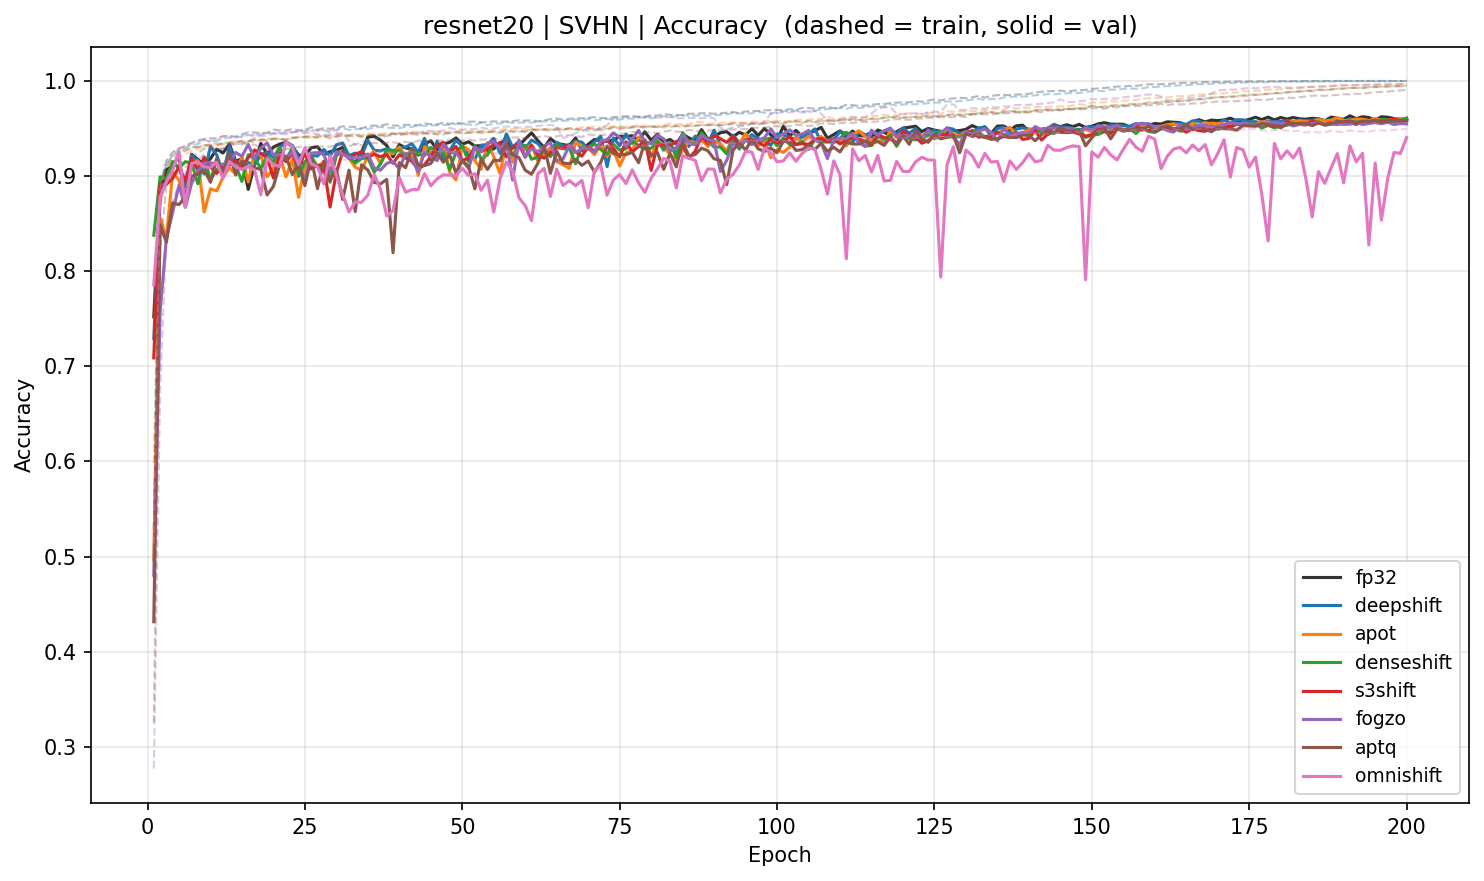
\includegraphics[width=\linewidth]{resnet20_svhn_acc.png}
\end{minipage}
\hfill
\begin{minipage}{0.48\textwidth}
  \centering
  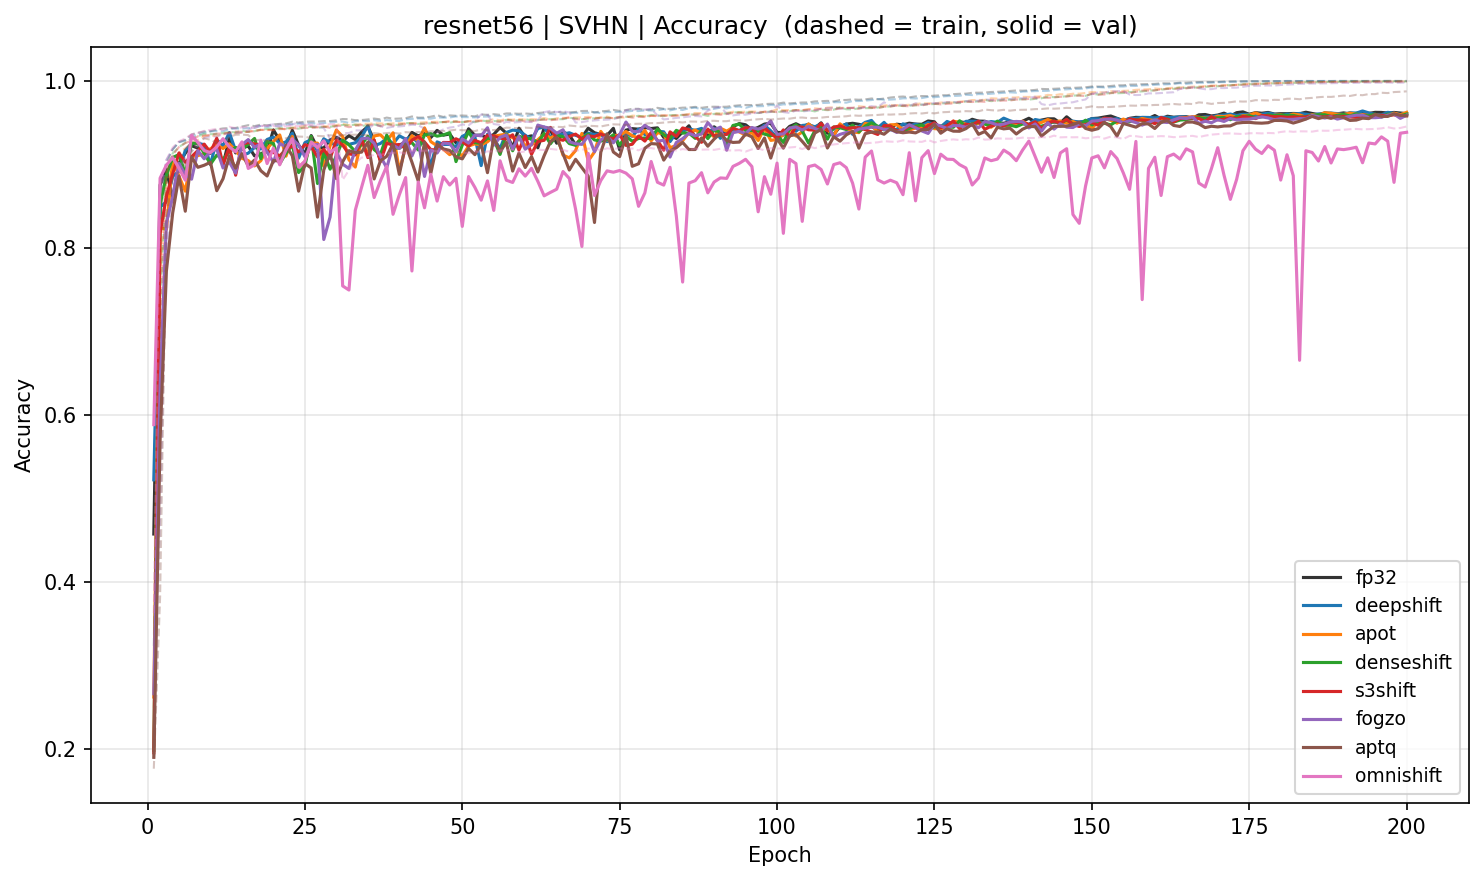
\includegraphics[width=\linewidth]{resnet56_svhn_acc.png}
\end{minipage}
\caption{Train and Validation accuracy curves on SVHN.}
\label{fig:svhn_acc}
\end{figure}

\begin{figure}[H]
\centering
\begin{minipage}{0.48\textwidth}
  \centering
  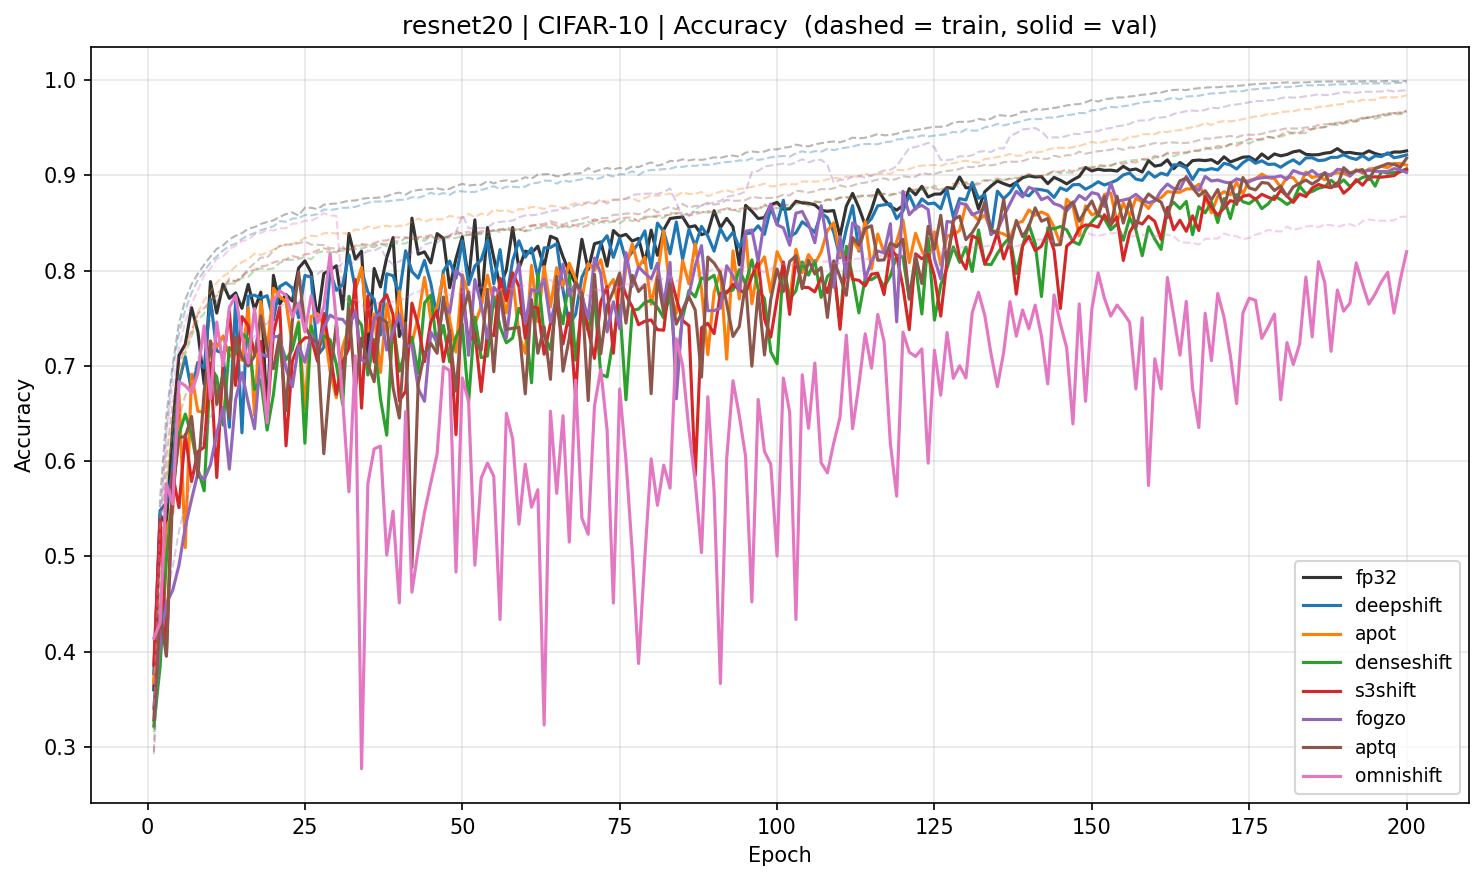
\includegraphics[width=\linewidth]{resnet20_cifar10_acc.png}
\end{minipage}
\hfill
\begin{minipage}{0.48\textwidth}
  \centering
  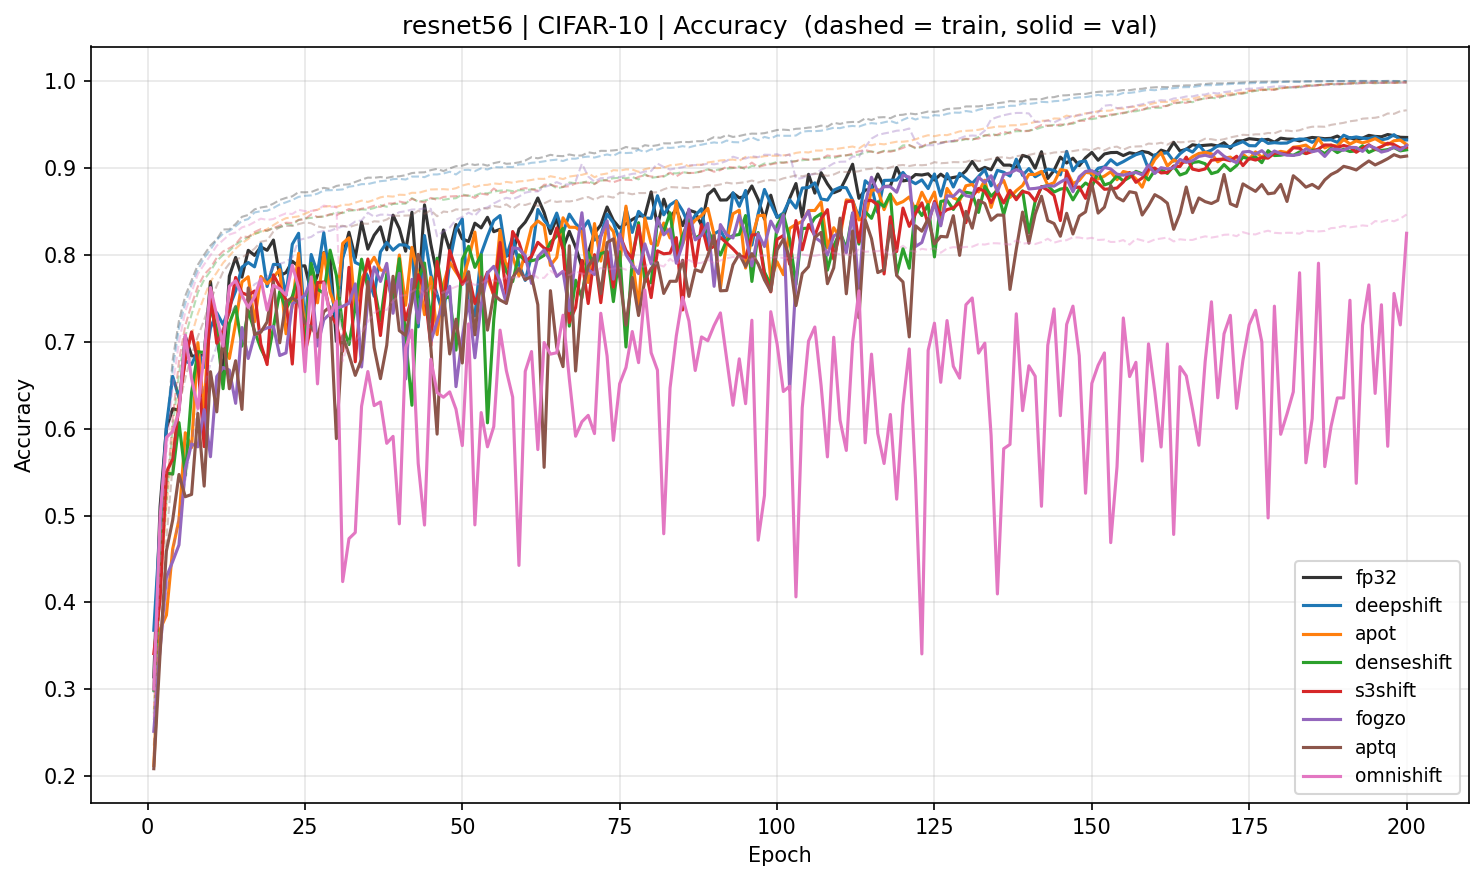
\includegraphics[width=\linewidth]{resnet56_cifar10_acc.png}
\end{minipage}
\caption{Train and Validation accuracy curves on CIFAR-10.}
\label{fig:cifar_acc}
\end{figure}

\begin{figure}[H]
\centering
\begin{minipage}{0.48\textwidth}
  \centering
  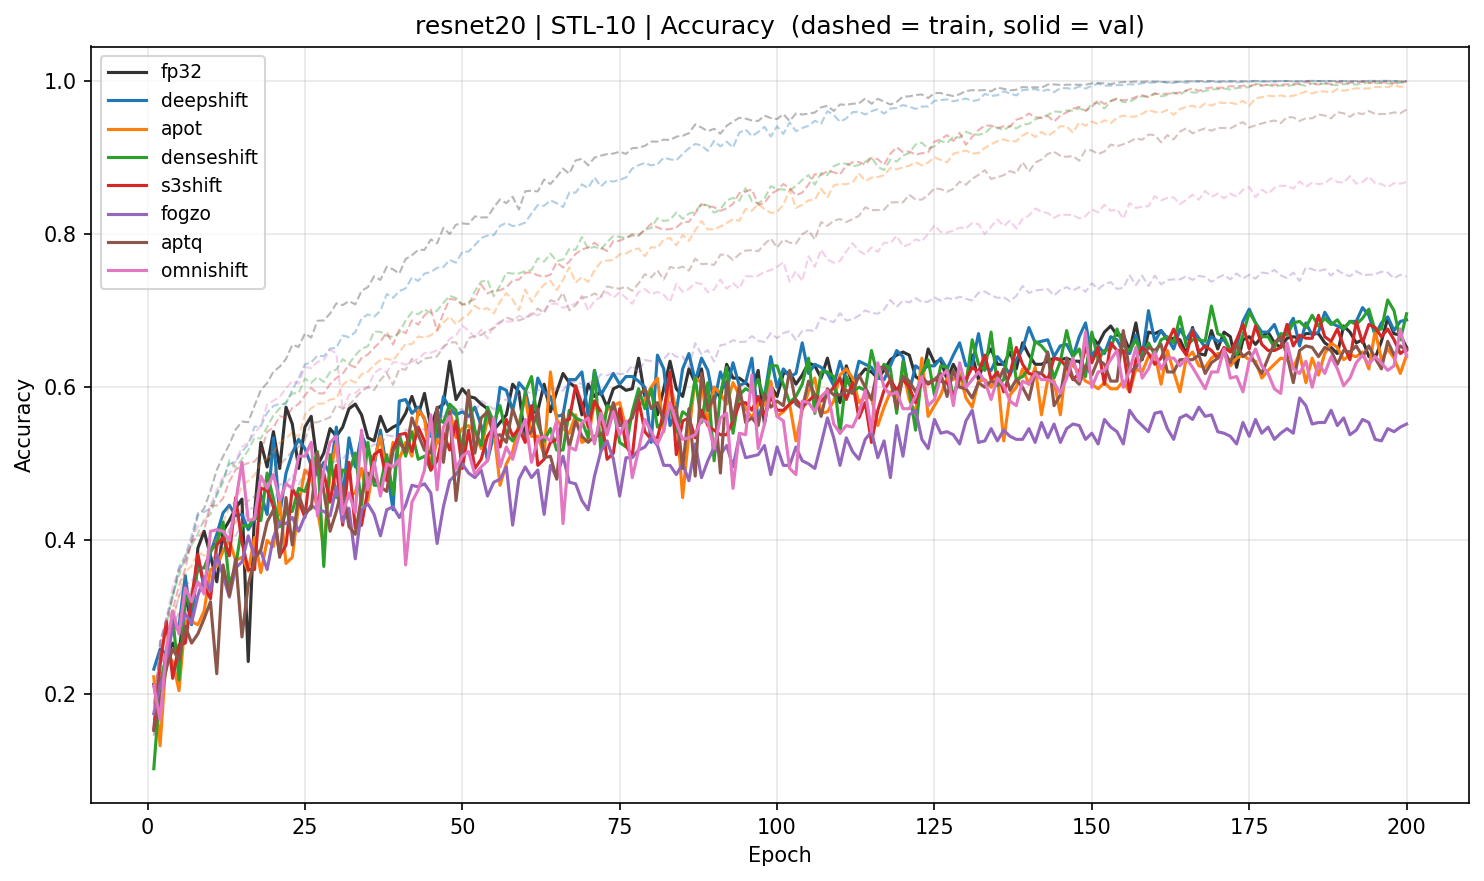
\includegraphics[width=\linewidth]{resnet20_stl10_acc.png}
\end{minipage}
\hfill
\begin{minipage}{0.48\textwidth}
  \centering
  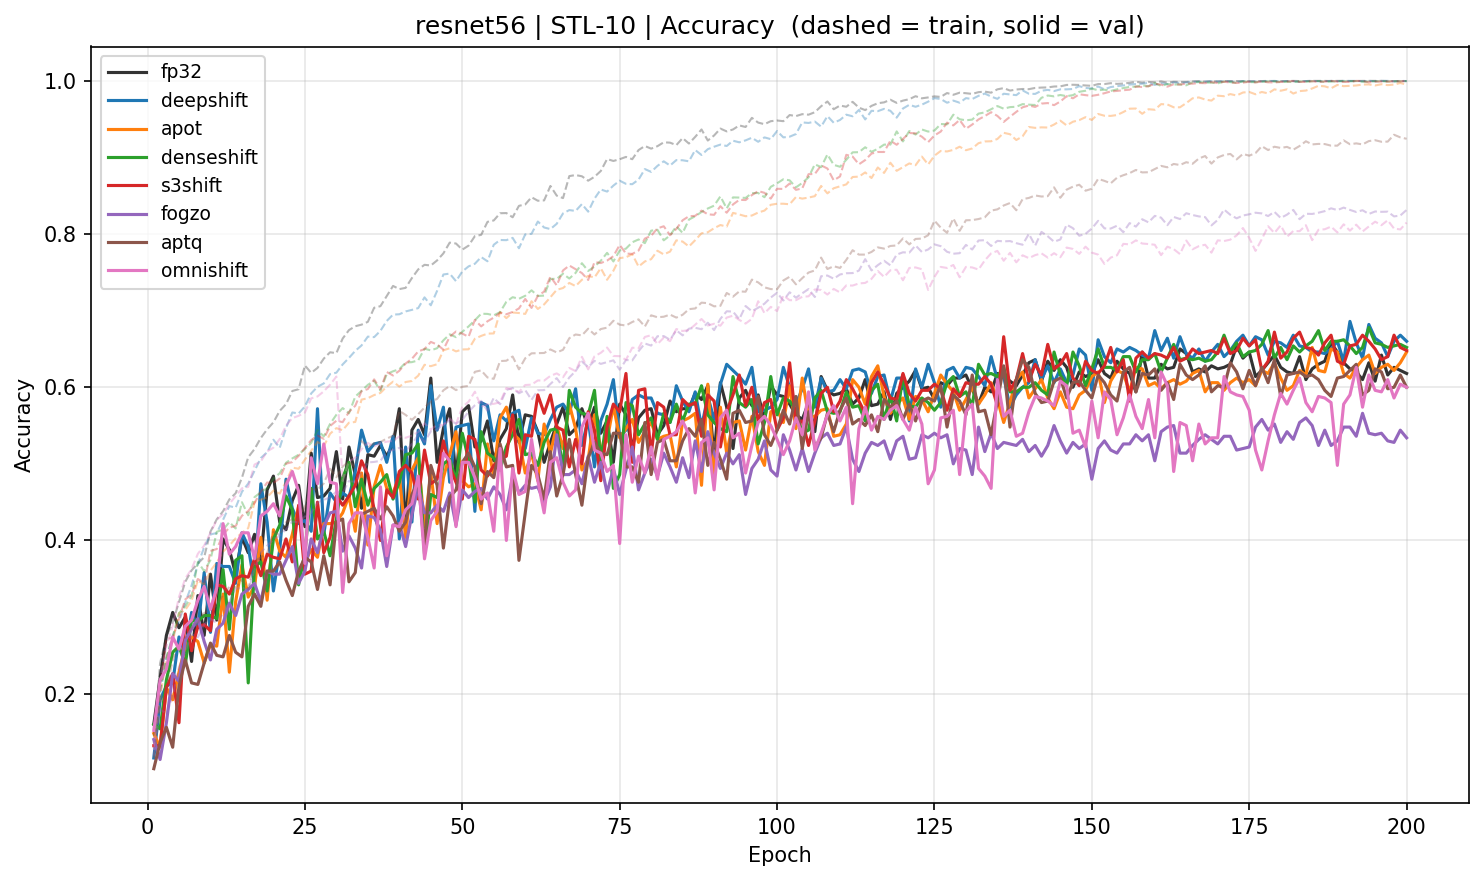
\includegraphics[width=\linewidth]{resnet56_stl10_acc.png}
\end{minipage}
\caption{Train and Validation accuracy curves on STL-10.}
\label{fig:stl_acc}
\end{figure}

\subsection{Ablation Study}
\label{sec:ablation}

Table~\ref{tab:ablation} traces the energy reduction on ResNet-20 as each constitutive component of \omnishift{} is added in isolation and in combination, evaluated with a fixed seed 42. Eight configurations span the complete design space from the FP32 baseline to the fully coordinated pipeline. All intermediate rows use learnable sparse gating where applicable; the two rightmost configurations in the final group test EWGS and PoT-Act independently before combining them in the full \omnishift{}.

\paragraph{Shift weights and learnable sparsity deliver the dominant energy gains.} Replacing FP32 multiplications with shift-based weights (row 2) achieves the 4.2$\times$ baseline. Introducing a learnable sparse gate without PoT-BN (row 4) amplifies this to 10.3$\times$ on CIFAR-10 and 17.7$\times$ on SVHN at near-lossless accuracy ($-0.11$~pp and $+0.25$~pp relative to FP32 respectively): the gate zeroes 62.9\% and 81.5\% of weights, entirely skipping the corresponding multiply-accumulate operations. Adding PoT-BN on top (row 5) eliminates BN-scale multiplications and contributes an additional incremental reduction to 11.2$\times$/19.1$\times$ at negligible accuracy cost. Together, sparse-shift weights and PoT-BN account for the structural majority of the final energy reduction.

\paragraph{EWGS amplifies sparsity without improving accuracy.} Introducing EWGS across all quantizers (row 6) changes CIFAR-10 accuracy by only $-0.12$~pp and SVHN by $-0.06$~pp relative to row 5, yet sparsity increases by $+11.6$~pp on CIFAR-10 (64.7\%$\to$76.2\%) and $+5.7$~pp on SVHN (81.7\%$\to$87.3\%), pushing energy to 15.6$\times$/25.2$\times$. The direction-aware gradient scaling of EWGS pushes marginal weights below the threshold $\tau$ faster under the existing classification loss; it does not improve the loss landscape for accuracy. Row 6 strictly dominates row 5 on all metrics: higher sparsity, lower energy, and near-equal accuracy.

\paragraph{PoT activations increase measured energy in isolation.} Row 7 applies PoT-act quantization without EWGS, making the datapath end-to-end multiply-free. Despite this, measured energy increases versus row 5 (0.0169$\to$0.0194~GpJ on CIFAR-10; 0.0099$\to$0.0127~GpJ on SVHN): the energy counter adds per-activation rounding operations at the output of each layer but cannot credit the shift-shift simplification in the downstream convolution, a conservative property of the current measurement model noted in Section~\ref{sec:method}. Simultaneously, sparsity falls (64.7\%$\to$58.8\% on CIFAR-10) as dual quantization of weights and activations disrupts the threshold learning dynamics. Row 7 is strictly dominated by row 6 on every metric.

\paragraph{EWGS and PoT-Act synergize in the full pipeline.} Combining both components (row 8, \omnishift{}) reverses the sparsity degradation observed in row 7: CIFAR-10 sparsity reaches 89.0\% ($+12.8$~pp vs row 6) and SVHN reaches 93.4\% ($+6.1$~pp), driving energy to 27.6$\times$/37.7$\times$. The EWGS-driven sparsity amplification counteracts the threshold disruption introduced by PoT-Act, producing a net sparsification effect that neither component achieves alone. The accuracy cost concentrates on CIFAR-10 ($-8.1$~pp vs row 6), while SVHN retains 94.78\% ($-1.6$~pp vs row 6). This asymmetry reflects the representational bottleneck of the 8-level PoT activation grid on high intra-class-variance data identified in Section~\ref{sec:experiments}.

\begin{table}[H]
\centering
\small
\caption{Component ablation on ResNet-20 (seed 42, learnable sparse mode). Each configuration adds one or more components to the prior design. E: energy (GpJ); Sp: weight sparsity (\%); $\times$: energy reduction vs FP32 (0.1887~GpJ). The \omnishift{} row matches Table~\ref{tab:r20} exactly.}
\label{tab:ablation}
\setlength{\tabcolsep}{4pt}
\begin{tabular}{@{}l rrrr rrrr@{}}
\toprule
& \multicolumn{4}{c}{CIFAR-10} & \multicolumn{4}{c}{SVHN} \\
\cmidrule(lr){2-5}\cmidrule(lr){6-9}
Configuration & Acc & E & Sp & $\times$ & Acc & E & Sp & $\times$ \\
\midrule
FP32                                         & 92.17 & 0.1887 &  0.0 &  1.0 & 96.82 & 0.1887 &  0.0 &  1.0 \\
Shift-W                                      & 92.13 & 0.0446 &  0.0 &  4.2 & 96.71 & 0.0446 &  0.0 &  4.2 \\
Shift-W + PoT-BN                             & 92.02 & 0.0438 &  0.0 &  4.3 & 96.42 & 0.0438 &  0.0 &  4.3 \\
Shift-W + SparseShift                        & 92.06 & 0.0184 & 62.9 & 10.3 & 96.46 & 0.0107 & 81.5 & 17.7 \\
Shift-W + SparseShift + PoT-BN               & 91.21 & 0.0169 & 64.7 & 11.2 & 96.45 & 0.0099 & 81.7 & 19.1 \\
Shift-W + SparseShift + PoT-BN + EWGS        & 91.09 & 0.0121 & 76.2 & 15.6 & 96.39 & 0.0075 & 87.3 & 25.2 \\
Shift-W + SparseShift + PoT-BN + PoT-Act     & 89.77 & 0.0194 & 58.8 &  9.7 & 96.02 & 0.0127 & 75.0 & 14.9 \\
\midrule
\omnishift{} (all: +EWGS +PoT-Act)           & 83.01 & \textbf{0.0068} & \textbf{89.0} & \textbf{27.6} & 94.78 & \textbf{0.0050} & \textbf{93.4} & \textbf{37.7} \\
\bottomrule
\end{tabular}
\end{table}

\subsection{Analysis}

The 48 controlled runs span three orders of magnitude in measured energy - from FP32 on ResNet-20 at 0.1887~GpJ down to \omnishift{} on ResNet-56/SVHN at 0.0053~GpJ - and reveal several cross-cutting patterns about how quantization strategies interact with data complexity, backbone depth, and sparsity.

\paragraph{The energy ceiling of dense shift quantization.} A defining feature common to both Tables~\ref{tab:r20} and~\ref{tab:r56} is the absolute uniformity among the five non-sparse baselines: DeepShift, APoT, DenseShift, S$^3$, and FOGZO all achieve exactly 4.2$\times$ on ResNet-20 and 4.3$\times$ on ResNet-56, regardless of differences in weight parameterization or gradient estimator. This ceiling follows directly from the energy model: a dense FP32 MAC costs $3.7 + 0.9 = 4.6$~pJ; its shift-quantized counterpart costs $0.13 + 0.9 = 1.03$~pJ, giving an intrinsic ratio of $4.6/1.03 \approx 4.47\times$. The measured 4.2$\times$ falls slightly short because the stem convolution and linear classifier, retained in full precision, account for approximately 2\% of ResNet-20 total energy at the FP32 rate. Without structural zeros, no quantization design can circumvent this bound. Within the dense group, DeepShift is the most accurate method overall, marginally exceeding FP32 on CIFAR-10 ($+0.06$~pp on ResNet-20, $+0.13$~pp on ResNet-56), consistent with the hypothesis that the logarithmic weight grid acts as implicit magnitude regularization. The ES values for the dense group (2,030-2,169 on ResNet-20 SVHN; 692-724 on ResNet-56) form a tight cluster reflecting their identical energy denominator; differences within the cluster are driven entirely by accuracy.

\paragraph{Emergent versus explicit sparsity.} APTQ and \omnishift{} are the only methods that surpass the 4.2$\times$ ceiling by producing structural zeros. APTQ achieves emergent sparsity - 74.9\%/84.6\% on CIFAR-10/SVHN for ResNet-20 - through the geometry of its two-sub-filter difference construction, without an explicit pruning objective \cite{frankle2019lottery,han2016deepcomp}, and delivers the best accuracy-energy tradeoff: 96.50\% at ES~=~10,266 on SVHN ($-0.32$~pp vs.\ FP32) and 91.35\% at ES~=~6,817 on CIFAR-10 ($-0.82$~pp). \omnishift{} instead forces explicit sparsity via a learned threshold $\tau$ \cite{louizos2018l0,molchanov2017pruning}, adding PoT-BN and PoT-Act for full multiply-free datapath coverage. This advances ES to 12,207/18,956 on ResNet-20 (CIFAR-10/SVHN) at larger accuracy costs ($-9.16$~pp CIFAR-10, $-2.04$~pp SVHN). The contrast delineates a core trade-off: emergent sparsity offers a smoother optimization landscape and superior accuracy retention; explicit joint-quantization is required to approach the ES values above 10,000 reached on SVHN.

\paragraph{Convergence dynamics.} The validation curves in Figure~\ref{fig:svhn_acc} reveal a convergence signature unique to \omnishift{}: while all other methods converge smoothly to stable plateaus on SVHN within 30-50 epochs, \omnishift{} (pink) exhibits large-amplitude periodic oscillations throughout the full 200-epoch schedule, with validation accuracy repeatedly dropping from a running mean of $\sim$95\% to 80-85\% before recovering. These oscillations arise from the discrete sparsity gate: as latent weights evolve under gradient updates, marginal weights near the threshold $\tau$ periodically cross the gate boundary in batches, abruptly changing the effective network topology. On CIFAR-10 (Figure~\ref{fig:cifar_acc}), the more diagnostically important observation is the persistent 9-10~pp gap between \omnishift{} and FP32: this gap is established early in training (by epoch $\sim$50) and does not narrow over the remaining 150 epochs, nor does it change when moving from ResNet-20 (left, $-9.2$~pp) to ResNet-56 (right, $-10.1$~pp). The depth-invariance of this gap distinguishes it from an optimization failure - which would show partial recovery with additional model capacity - and points instead to a representational bottleneck imposed by the 8-level PoT activation grid.

\paragraph{STL-10 and low-data sensitivity.} Figure~\ref{fig:stl_acc} shows qualitatively different dynamics: all validation curves exhibit high variance throughout training due to the small 5,000-image training set, and train-validation gaps reach 30-35~pp by epoch 200, indicating strong overfitting across all methods. DenseShift (green) and S$^3$ (red) trend above FP32 in final accuracy (68.46\% and 68.11\% vs.\ 67.63\% FP32 on ResNet-20), reinforcing the hypothesis that PoT weight grids provide regularization beneficial under data scarcity \cite{liu2019rethinkpruning}. \omnishift{} broadly tracks the main cluster on ResNet-20 (65.93\%) but falls further below on ResNet-56 (60.62\%), a substantially larger depth-induced accuracy regression than on CIFAR-10 or SVHN. FOGZO (purple) is the clearest outlier: its validation curve separates from the main cluster around epoch 30-50 and fails to recover (59.03\%/56.23\% on ResNet-20/56), while FOGZO's train curve also lags the group, confirming that ZO perturbations are harmful in this data-scarce regime. The ES values on STL-10 are systematically lower than on SVHN or CIFAR-10 because the higher energy denominator from lower sparsity (64.3\%/73.8\% vs.\ 93.4\%/98.0\% on SVHN) raises absolute energy; \omnishift{}'s ES of 3,856 on ResNet-20/STL-10 is still 10.8$\times$ the FP32 baseline (358), but is only a fifth of the SVHN ES.

\paragraph{Backbone scaling and super-linear energy efficiency.} Moving from ResNet-20 to ResNet-56 increases the FP32 energy baseline by $3.1\times$ (0.1887 to 0.5809~GpJ). For \omnishift{}, however, the absolute quantized energy remains essentially constant: 0.0068 vs.\ 0.0067~GpJ on CIFAR-10, and 0.0050 vs.\ 0.0053~GpJ on SVHN - changes of less than 6\%. This near-constant absolute energy arises because weight sparsity deepens substantially in the deeper backbone: 89.0\%$\to$96.9\% on CIFAR-10 and 93.4\%$\to$98.0\% on SVHN. Combined with the $3.1\times$ larger FP32 denominator, the ES values scale proportionally: CIFAR-10 from 12,207 to 12,476 (roughly constant absolute energy), and SVHN from 18,956 to 17,930 - both remaining orders of magnitude above the dense-shift cluster. The energy reduction ratio improves as 27.6$\times$$\to$87.0$\times$ on CIFAR-10 and 37.7$\times$$\to$109.7$\times$ on SVHN, closely tracking the $3.1\times$ baseline scaling factor.

\paragraph{Hardware multiplication demand.} Table~\ref{tab:dsp} reports DSP demand under the Artix-7 FPGA model. All dense shift methods retain standard BN and therefore include BN-scale multiply operations, giving $N_\text{mul} = 0.644\times10^{-3}$~G on ResNet-20 and $0.988\times10^{-3}$~G on ResNet-56 - the increase with depth reflects the additional BN layers in the 9-block stages. \omnishift{}'s PoT-BN eliminates all BN multiplications, leaving only the 3$\times$3 stem ($3\to16$~ch, $32\times32$) and the linear classifier for a total of $N_\text{mul} = 0.443\times10^{-3}$~G - \emph{constant} across backbone depths. Consequently, the DSP demand for \omnishift{} is 1,772k on both ResNet-20 and ResNet-56, while that of the non-PoT-BN shift methods grows from 2,575k to 3,951k. The resulting DSP reduction versus FP32 is 92.6$\times$ on ResNet-20 and \textbf{285.1$\times$} on ResNet-56, compared to 63.7$\times$ and 128.0$\times$ for the other shift methods. This constant-$N_\text{mul}$ property is a structural consequence of PoT-BN: for deeper backbones, the growing BN-multiply contribution that limits all other methods is entirely avoided, so \omnishift{}'s DSP advantage grows linearly with depth.

\begin{table}[H]
\centering
\small
\caption{DSP48E2 demand on Xilinx Artix-7 XC7A200T (740 physical DSPs). $D = 4\,N_\text{mul}$ per forward pass. \omnishift{} uses PoT-BN and thus has no BN multiplications; $N_\text{mul}$ stays constant across backbone depths. All other shift methods retain standard BN.}
\label{tab:dsp}
\setlength{\tabcolsep}{5pt}
\begin{tabular}{@{} >{\raggedright\arraybackslash}p{5.6cm} rr rr @{}}
\toprule
& \multicolumn{2}{c}{ResNet-20} & \multicolumn{2}{c}{ResNet-56} \\
\cmidrule(lr){2-3}\cmidrule(lr){4-5}
Method & $N_\text{mul}$ (G) & DSP red.\ $\downarrow$ & $N_\text{mul}$ (G) & DSP red.\ $\downarrow$ \\
\midrule
FP32                     & 0.0410  & 1.0$\times$   & 0.1263  & 1.0$\times$ \\
DeepShift / APoT / DenseShift / S$^3$ / FOGZO / APTQ & 0.000644 & 63.7$\times$ & 0.000988 & 128.0$\times$ \\
\omnishift{} (PoT-BN)   & \textbf{0.000443} & \textbf{92.6$\times$}  & \textbf{0.000443} & \textbf{285.1$\times$} \\
\bottomrule
\end{tabular}
\end{table}

\section{Conclusion}
\label{sec:conclusion}

We presented \omnishift{}, a training framework that achieves fully multiply-free CNN inference by coordinating power-of-two quantization across weights, Batch Normalization scales, and activations simultaneously. Through a factory-based dependency injection design, the framework requires zero architectural changes to apply to any backbone, as demonstrated across ResNet-20 and ResNet-56 on three datasets. On ResNet-56 with SVHN, \omnishift{} achieves $\mathbf{109.7\times}$ energy reduction versus full-precision at 95.03\% accuracy and 98.0\% sparsity - the highest energy efficiency we are aware of for shift-based CNN quantization. The efficiency score reaches 17,930 (Acc\%/GpJ), versus 167 for FP32 on the same backbone and dataset, a 107$\times$ improvement. The backbone scaling analysis confirms that energy reduction ratios grow proportionally with model depth while absolute quantized energy remains near-constant, validating the generalizability of the approach.

Our ablation study reveals two key findings: (1) the dominant energy gain comes from learnable sparse-shift quantization, not from PoT activations; and (2) EWGS's primary role in this setting is sparsity amplification (up to $+11.6$~pp), not gradient quality improvement. The hardware analysis shows that PoT-BN provides a structural benefit beyond energy: by eliminating all BN multiplications, \omnishift{}'s DSP demand is constant regardless of backbone depth (0.000443~G), yielding 285.1$\times$ DSP reduction on ResNet-56 versus 128.0$\times$ for the other shift methods.

\paragraph{Limitations.}
The main accuracy limitation is a significant CIFAR-10 regression: $-9.2$~pp on ResNet-20 and $-10.1$~pp on ResNet-56. The depth-invariance of this gap across both backbones and its absence on SVHN ($-2.0$~pp) identify it as a representational bottleneck of the 8-level PoT activation grid on high intra-class-variance data, rather than an optimization failure. A second limitation is training instability inherent to the learnable sparse-shift formulation. The validation accuracy of the full \omnishift{} pipeline exhibits large-amplitude periodic oscillations throughout the 200-epoch schedule: populations of marginal weights near the gate threshold $\tau$ cross the sparsity boundary in synchronized batches, temporarily disrupting the effective network topology and causing transient accuracy drops of 10-15~pp before recovery. This instability is more pronounced on ResNet-56, where a larger parameter space means more weights simultaneously near threshold; it increases the risk of early stopping at a trough and requires careful checkpoint selection from the running mean rather than the instantaneous validation value.

\paragraph{Future work.}
Three directions are planned. First, stabilizing the learnable-threshold training dynamics through threshold annealing schedules or moving-average gate updates that prevent synchronized boundary crossings, aiming to produce smooth convergence curves comparable to the dense shift baselines. Second, recovering the CIFAR-10 accuracy gap through knowledge distillation \cite{han2016deepcomp} from a full-precision teacher, which has shown 5-8~pp recovery in comparable sparse quantization settings; this is expected to close most of the $-9$ to $-10$~pp gap while preserving the energy advantage. Third, generalizing \omnishift{} beyond CIFAR-style ResNets to wider CNN families (MobileNet, EfficientNet) and ultimately Vision Transformers, where the multi-head self-attention matmul is the dominant multiply source and PoT quantization of the key-query product represents the next frontier in multiply-free deployment.

\begin{thebibliography}{99}

\bibitem{chen2020adder}
H.\ Chen, Y.\ Wang, C.\ Xu, B.\ Shi, C.\ Xu, Q.\ Tian, and C.\ Xu,
``AdderNet: Do we really need multiplications in deep learning?''
in \textit{Adv.\ Neural Inf.\ Process.\ Syst.\ (NeurIPS)}, 2020.

\bibitem{courbariaux2015binaryconnect}
M.\ Courbariaux, Y.\ Bengio, and J.-P.\ David,
``BinaryConnect: Training deep neural networks with binary weights during propagations,''
in \textit{Adv.\ Neural Inf.\ Process.\ Syst.\ (NeurIPS)}, 2015.

\bibitem{rastegari2016xnor}
M.\ Rastegari, V.\ Ordonez, J.\ Redmon, and A.\ Farhadi,
``XNOR-Net: ImageNet classification using binary convolutional neural networks,''
in \textit{Proc.\ ECCV}, 2016.

\bibitem{li2016twn}
F.\ Li, B.\ Zhang, and B.\ Liu,
``Ternary weight networks,''
in \textit{NIPS Workshop on Efficient Methods for Deep Neural Networks}, 2016.

\bibitem{zhu2016ttq}
C.\ Zhu, S.\ Han, H.\ Mao, and W.\ J.\ Dally,
``Trained ternary quantization,''
in \textit{Proc.\ ICLR}, 2017.

\bibitem{elhoushi2021deepshift}
M.\ Elhoushi, Z.\ Chen, F.\ Shafiq, Y.\ H.\ Tian, and J.\ R.\ Li,
``DeepShift: Towards multiplication-less neural networks,''
in \textit{Proc.\ IEEE/CVF CVPR Workshops}, 2021.

\bibitem{li2020apot}
Y.\ Li, R.\ Dong, and W.\ Wang,
``Additive powers-of-two quantization: An efficient non-uniform discretization for neural networks,''
in \textit{Proc.\ ICLR}, 2020.

\bibitem{banner2018pobn}
R.\ Banner, I.\ Nahshan, E.\ Hoffer, and D.\ Soudry,
``Post-training 4-bit quantization of convolution networks for rapid-deployment,''
in \textit{Adv.\ Neural Inf.\ Process.\ Syst.\ (NeurIPS)}, 2019.

\bibitem{esser2020lsq}
S.\ K.\ Esser, J.\ L.\ McKinstry, D.\ Bablani, R.\ Appuswamy, and D.\ S.\ Modha,
``Learned step size quantization,''
in \textit{Proc.\ ICLR}, 2020.

\bibitem{zhang2018lq}
D.\ Zhang, J.\ Yang, D.\ Ye, and G.\ Hua,
``LQ-Nets: Learned quantization for highly accurate and compact deep neural networks,''
in \textit{Proc.\ ECCV}, 2018.

\bibitem{lee2021ewgs}
D.-H.\ Lee, S.\ Kim, K.\ Kim, and S.\ Hwang,
``Network quantization with element-wise gradient scaling,''
in \textit{Proc.\ IEEE/CVF CVPR}, 2021.

\bibitem{bengio2013ste}
Y.\ Bengio, N.\ L\'{e}onard, and A.\ Courville,
``Estimating or propagating gradients through stochastic neurons for conditional computation,''
in \textit{NIPS Workshop on Deep Learning}, 2013.

\bibitem{li2023denseshift}
Z.\ Li, H.\ Li, and B.\ Zhuang,
``DenseShift: Towards accurate and efficient low-bit power-of-two quantization,''
in \textit{Proc.\ IEEE/CVF ICCV}, 2023.

\bibitem{li2021s3}
Y.\ Li, C.\ Gong, X.\ Tan, Y.\ Yang, J.\ Meng, and J.\ Yuan,
``$\text{S}^3$: Sign-sparse-shift reparametrization for effective training of low-bit shift networks,''
in \textit{Adv.\ Neural Inf.\ Process.\ Syst.\ (NeurIPS)}, 2021.

\bibitem{liu2024aptq}
Z.\ Liu, B.\ Liu, and R.\ Li,
``Asymmetric power-of-two quantization for shift networks,''
\textit{Sensors}, vol.\ 24, no.\ 1, p.\ 181, 2024.

\bibitem{hubara2016bnn}
I.\ Hubara, M.\ Courbariaux, D.\ Soudry, R.\ El-Yaniv, and Y.\ Bengio,
``Binarized neural networks,''
in \textit{Adv.\ Neural Inf.\ Process.\ Syst.\ (NeurIPS)}, 2016.

\bibitem{guo2019dsq}
R.\ Guo, X.\ Liu, J.\ Chen, W.\ Hu, J.\ Cao, J.\ Yu, and J.\ Han,
``Differentiable soft quantization: Bridging full-precision and low-bit neural networks,''
in \textit{Proc.\ IEEE/CVF ICCV}, 2019.

\bibitem{chen2025fogzo}
K.\ Chen \textit{et al.},
``FOGZO: Zeroth-order optimization for training shift networks,''
in \textit{Adv.\ Neural Inf.\ Process.\ Syst.\ (NeurIPS)}, 2025.

\bibitem{jacob2018quantization}
B.\ Jacob, S.\ Kligys, B.\ Chen, M.\ Zhu, M.\ Tang, A.\ Howard, H.\ Adam, and D.\ Kalenichenko,
``Quantization and training of neural networks for efficient integer-arithmetic-only inference,''
in \textit{Proc.\ IEEE/CVF CVPR}, 2018.

\bibitem{nagel2019datafree}
M.\ Nagel, M.\ van Baalen, T.\ Blankevoort, and M.\ Welling,
``Data-free quantization through weight equalization and bias correction,''
in \textit{Proc.\ IEEE/CVF ICCV}, 2019.

\bibitem{zhou2017inq}
A.\ Zhou, A.\ Yao, Y.\ Guo, L.\ Xu, and Y.\ Chen,
``Incremental network quantization: Towards lossless CNNs with low-precision weights,''
in \textit{Proc.\ ICLR}, 2017.

\bibitem{krizhevsky2009}
A.\ Krizhevsky,
``Learning multiple layers of features from tiny images,''
Tech.\ Rep., University of Toronto, 2009.

\bibitem{netzer2011}
Y.\ Netzer, T.\ Wang, A.\ Coates, A.\ Bissacco, B.\ Wu, and A.\ Y.\ Ng,
``Reading digits in natural images with unsupervised feature learning,''
in \textit{NIPS Workshop on Deep Learning and Unsupervised Feature Learning}, 2011.

\bibitem{coates2011}
A.\ Coates, H.\ Lee, and A.\ Y.\ Ng,
``An analysis of single-layer networks in unsupervised feature learning,''
in \textit{Proc.\ AISTATS}, 2011.

\bibitem{he2016resnet}
K.\ He, X.\ Zhang, S.\ Ren, and J.\ Sun,
``Deep residual learning for image recognition,''
in \textit{Proc.\ IEEE/CVF CVPR}, 2016.

\bibitem{micikevicius2018mixed}
P.\ Micikevicius, S.\ Narang, J.\ Alben, G.\ Diamos, E.\ Elsen, D.\ Garcia, B.\ Ginsburg, M.\ Houston, O.\ Kuchaiev, G.\ Venkatesh, and H.\ Wu,
``Mixed precision training,''
in \textit{Proc.\ ICLR}, 2018.

\bibitem{horowitz2014energy}
M.\ Horowitz,
``1.1 Computing's energy problem (and what we can do about it),''
in \textit{Proc.\ IEEE Int.\ Solid-State Circuits Conf.\ (ISSCC)}, 2014.

\bibitem{frankle2019lottery}
J.\ Frankle and M.\ Carlin,
``The lottery ticket hypothesis: Finding sparse, trainable neural networks,''
in \textit{Proc.\ ICLR}, 2019.

\bibitem{han2016deepcomp}
S.\ Han, H.\ Mao, and W.\ J.\ Dally,
``Deep compression: Compressing deep neural networks with pruning, trained quantization and Huffman coding,''
in \textit{Proc.\ ICLR}, 2016.

\bibitem{louizos2018l0}
C.\ Louizos, M.\ Welling, and D.\ P.\ Kingma,
``Learning sparse neural networks through $L_0$ regularization,''
in \textit{Proc.\ ICLR}, 2018.

\bibitem{molchanov2017pruning}
P.\ Molchanov, S.\ Tyree, T.\ Karras, T.\ Aila, and J.\ Kautz,
``Pruning convolutional neural networks for resource efficient inference,''
in \textit{Proc.\ ICLR}, 2017.

\bibitem{liu2019rethinkpruning}
Z.\ Liu, M.\ Sun, T.\ Zhou, G.\ Huang, and T.\ Darrell,
``Rethinking the value of network pruning,''
in \textit{Proc.\ ICLR}, 2019.

\end{thebibliography}
\end{document}
